        \subsection{signals}

\begin{frame}{audio signals}{categorization}
	\begin{itemize}
		\item	\textbf{deterministic signals}:\\
				\textit{predictable}: future shape of the signal can be known (example: sinusoidal)
		\pause		
		\item	\textbf{random signals}:\\
				\textit{unpredictable}: no knowledge can help to predict what is coming next (example: white noise)
	\end{itemize}
	
	Every ``real-world'' audio signal can be modeled as a time-varying combination of 
	\begin{itemize}
		\item	(quasi-)periodic parts
		\item	(quasi-)random parts
	\end{itemize}
\end{frame}

\begin{frame}{audio signals}{periodic signals 1/3}
	\vspace{-5mm}
    periodic signals most prominent examples of deterministic signals: 
	\begin{eqnarray}
		x(t) 	&=& x(t+T_0)\nonumber\\
		f_0 	&=& \frac{1}{T_0}\nonumber\\
		\omega_0&=& \frac{2\pi}{T_0}\nonumber
	\end{eqnarray}
	\vspace{-10mm}
	\pause
	
	\begin{figure}
		\centering
			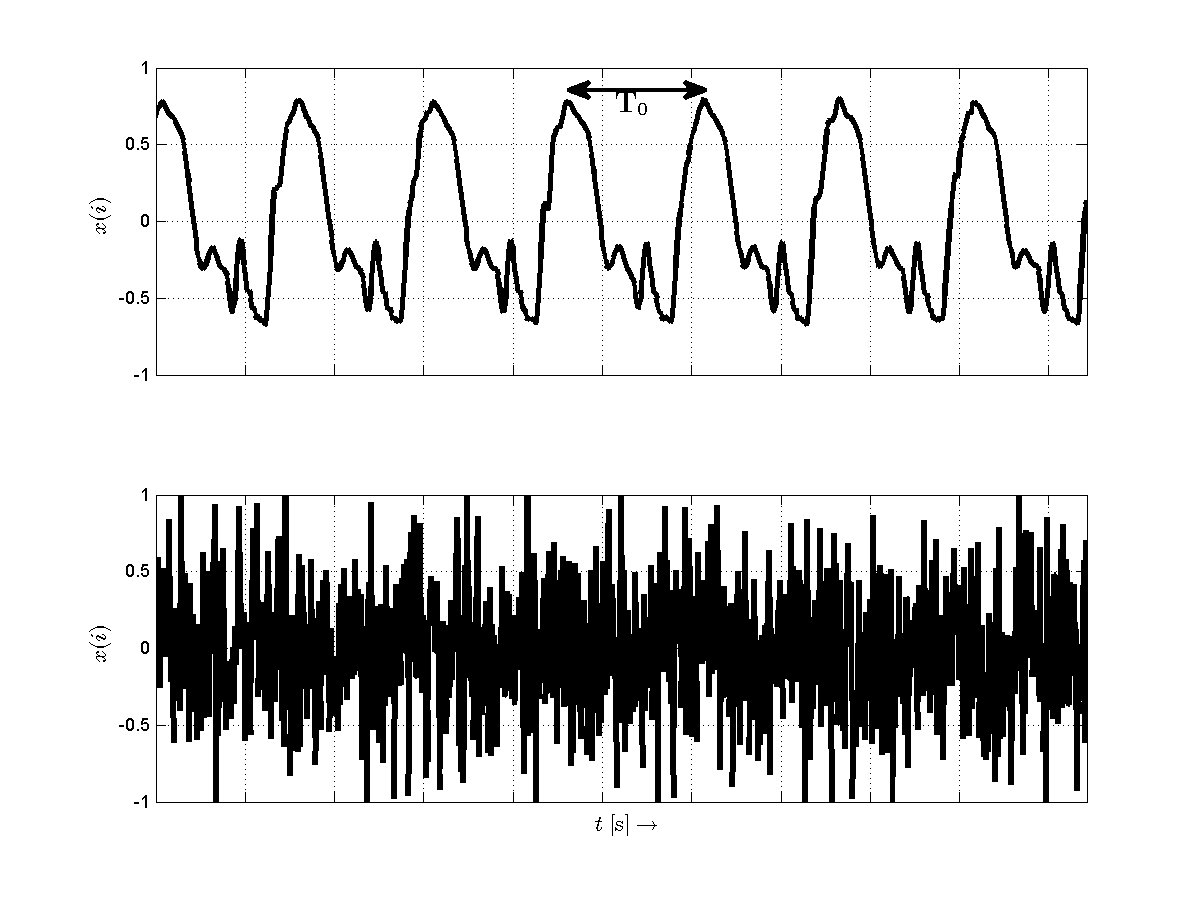
\includegraphics[height=5cm,width=\textwidth]{graph/periodic}
	\end{figure}
\end{frame}

\begin{frame}{audio signals}{periodic signals 2/3}
    \vspace{-5mm}
    \begin{block}{reconstruction}
    	periodic signals can be reconstructed through a sum of sinusoidals at frequencies $k\cdot\omega_0$
    \end{block}
    \only<1>{\vspace{70mm}}
    \vspace{-5mm}
	\setcounter{i}{1}
	\whiledo{\value{i}<6}	
	{
		\pause
		\only<\value{beamerpauses}>
		{
        
        
            \only<2>{
            \begin{equation}\nonumber
                \hat{x}(t) = a_1\cdot sin(\omega_0 t)
            \end{equation}}
            \only<3>{
            \begin{equation}\nonumber
                \hat{x}(t) = a_1\cdot sin(\omega_0 t) + a_2\cdot sin(2\cdot\omega_0 t)+\ldots+ a_{3}\cdot sin(3\cdot\omega_0 t)
            \end{equation}}
            \only<4>{
            \begin{equation}\nonumber
                \hat{x}(t) = a_1\cdot sin(\omega_0 t) + a_2\cdot sin(2\cdot\omega_0 t)+\ldots+ a_{10}\cdot sin(10\cdot\omega_0 t)
            \end{equation}}
            \only<5>{
            \begin{equation}\nonumber
                \hat{x}(t) = a_1\cdot sin(\omega_0 t) + a_2\cdot sin(2\cdot\omega_0 t)+\ldots+ a_{25}\cdot sin(25\cdot\omega_0 t)
            \end{equation}}
            \only<6>{
            \begin{equation}\nonumber
                \hat{x}(t) = a_1\cdot sin(\omega_0 t) + a_2\cdot sin(2\cdot\omega_0 t)+\ldots+ a_{50}\cdot sin(50\cdot\omega_0 t)
            \end{equation}}
			\vspace{-10mm}
            \begin{figure}
			\centering
                %\includemovie[poster=graph/additivesynthesis_saw_\arabic{i}.pdf,autoplay=true]{\textwidth}{4cm}{audio/additivesynthesis_saw_\arabic{i}.mp3}
                \includegraphics[width=\textwidth, height=4cm]{graph/additivesynthesis_saw_\arabic{i}.pdf}
			\end{figure}
            \vspace{-5mm}
			\begin{figure}
			\flushright
                \includemedia[
                    addresource=audio/additivesynthesis_saw_\arabic{i}.mp3,
                    width=.3\textwidth,
                    height=3mm,
                    activate=pageopen,
                    flashvars={
                        source=audio/additivesynthesis_saw_\arabic{i}.mp3  
                        &autoPlay=true
                    }]
                    {}
                    {APlayer.swf}
			\end{figure}
		}
		\stepcounter{i} 
	}	
	\setcounter{i}{1}
	\whiledo{\value{i}<6}	
	{
		\pause
		\only<\value{beamerpauses}>
		{
        
            \only<7>{
            \begin{equation}\nonumber
                \hat{x}(t) = a_1\cdot sin(\omega_0 t)
            \end{equation}}
            \only<8>{
            \begin{equation}\nonumber
                \hat{x}(t) = a_1\cdot sin(\omega_0 t) + a_3\cdot sin(3\cdot\omega_0 t)+\ldots+ a_{5}\cdot sin(5\cdot\omega_0 t)
            \end{equation}}
            \only<9>{
            \begin{equation}\nonumber
                \hat{x}(t) = a_1\cdot sin(\omega_0 t) + a_3\cdot sin(3\cdot\omega_0 t)+\ldots+ a_{19}\cdot sin(19\cdot\omega_0 t)
            \end{equation}}
            \only<10>{
            \begin{equation}\nonumber
                \hat{x}(t) = a_1\cdot sin(\omega_0 t) + a_3\cdot sin(3\cdot\omega_0 t)+\ldots+ a_{49}\cdot sin(49\cdot\omega_0 t)
            \end{equation}}
            \only<11>{
            \begin{equation}\nonumber
                \hat{x}(t) = a_1\cdot sin(\omega_0 t) + a_3\cdot sin(3\cdot\omega_0 t)+\ldots+ a_{99}\cdot sin(99\cdot\omega_0 t)
            \end{equation}}
            \vspace{-10mm}
			\begin{figure}
			\centering
                %\includemovie[poster=graph/additivesynthesis_rect_\arabic{i}.pdf,autoplay=true]{\textwidth}{4cm}{audio/additivesynthesis_rect_\arabic{i}.mp3}
                \includegraphics[width=\textwidth, height=4cm]{graph/additivesynthesis_rect_\arabic{i}.pdf}
 			\end{figure}
            \vspace{-5mm}
            \begin{figure}
			\flushright
               \includemedia[
                    addresource=audio/additivesynthesis_rect_\arabic{i}.mp3,
                    width=.3\textwidth,
                    height=3mm,
                    activate=pageopen,
                    flashvars={
                        source=audio/additivesynthesis_rect_\arabic{i}.mp3  
                        &autoPlay=true
                    }]
                    {}
                    {APlayer.swf}

 			\end{figure}
		}
		\stepcounter{i} 
	}	
\end{frame}

\begin{frame}{audio signals}{periodic signals 3/3}
    youtube --- mechanical additive synthesis:
    
    \url{http://youtu.be/8KmVDxkia_w}
    
\end{frame}


	
\begin{frame}{audio signals}{random process}
	\textbf{Random process}: ensemble of random series
	\begin{figure}
		\centering
			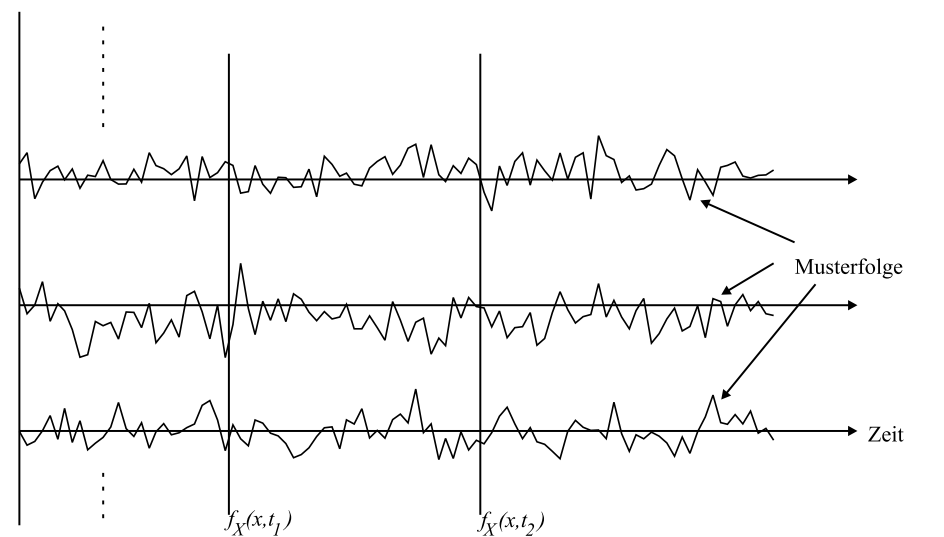
\includegraphics[scale=.25]{graph/randomprocess}
	\end{figure}
	\pause
	Special Cases:
	\begin{itemize}
		\item	\textbf{Stationarity}: all parameters (such as the mean) are time invariant
		\item	\textbf{Ergodicity}: process with equal time and ensemble mean (implies stationarity)
	\end{itemize}
\end{frame}
	
